% Editable vector version of distance-0.png.
% Regenerate from this directory:
% latex -interaction=nonstopmode -halt-on-error distance-0.tex
% dvisvgm --no-fonts --exact --bbox=papersize --output=distance-0.svg distance-0.dvi
\documentclass[tikz,border=0pt]{standalone}
\usepackage[T1]{fontenc}
\usepackage{newtxtext,newtxmath}
\usetikzlibrary{calc}
\definecolor{edgeblue}{RGB}{27,93,169}
\definecolor{diagonalred}{RGB}{195,39,44}
\definecolor{diagonalgreen}{RGB}{42,119,49}
\begin{document}
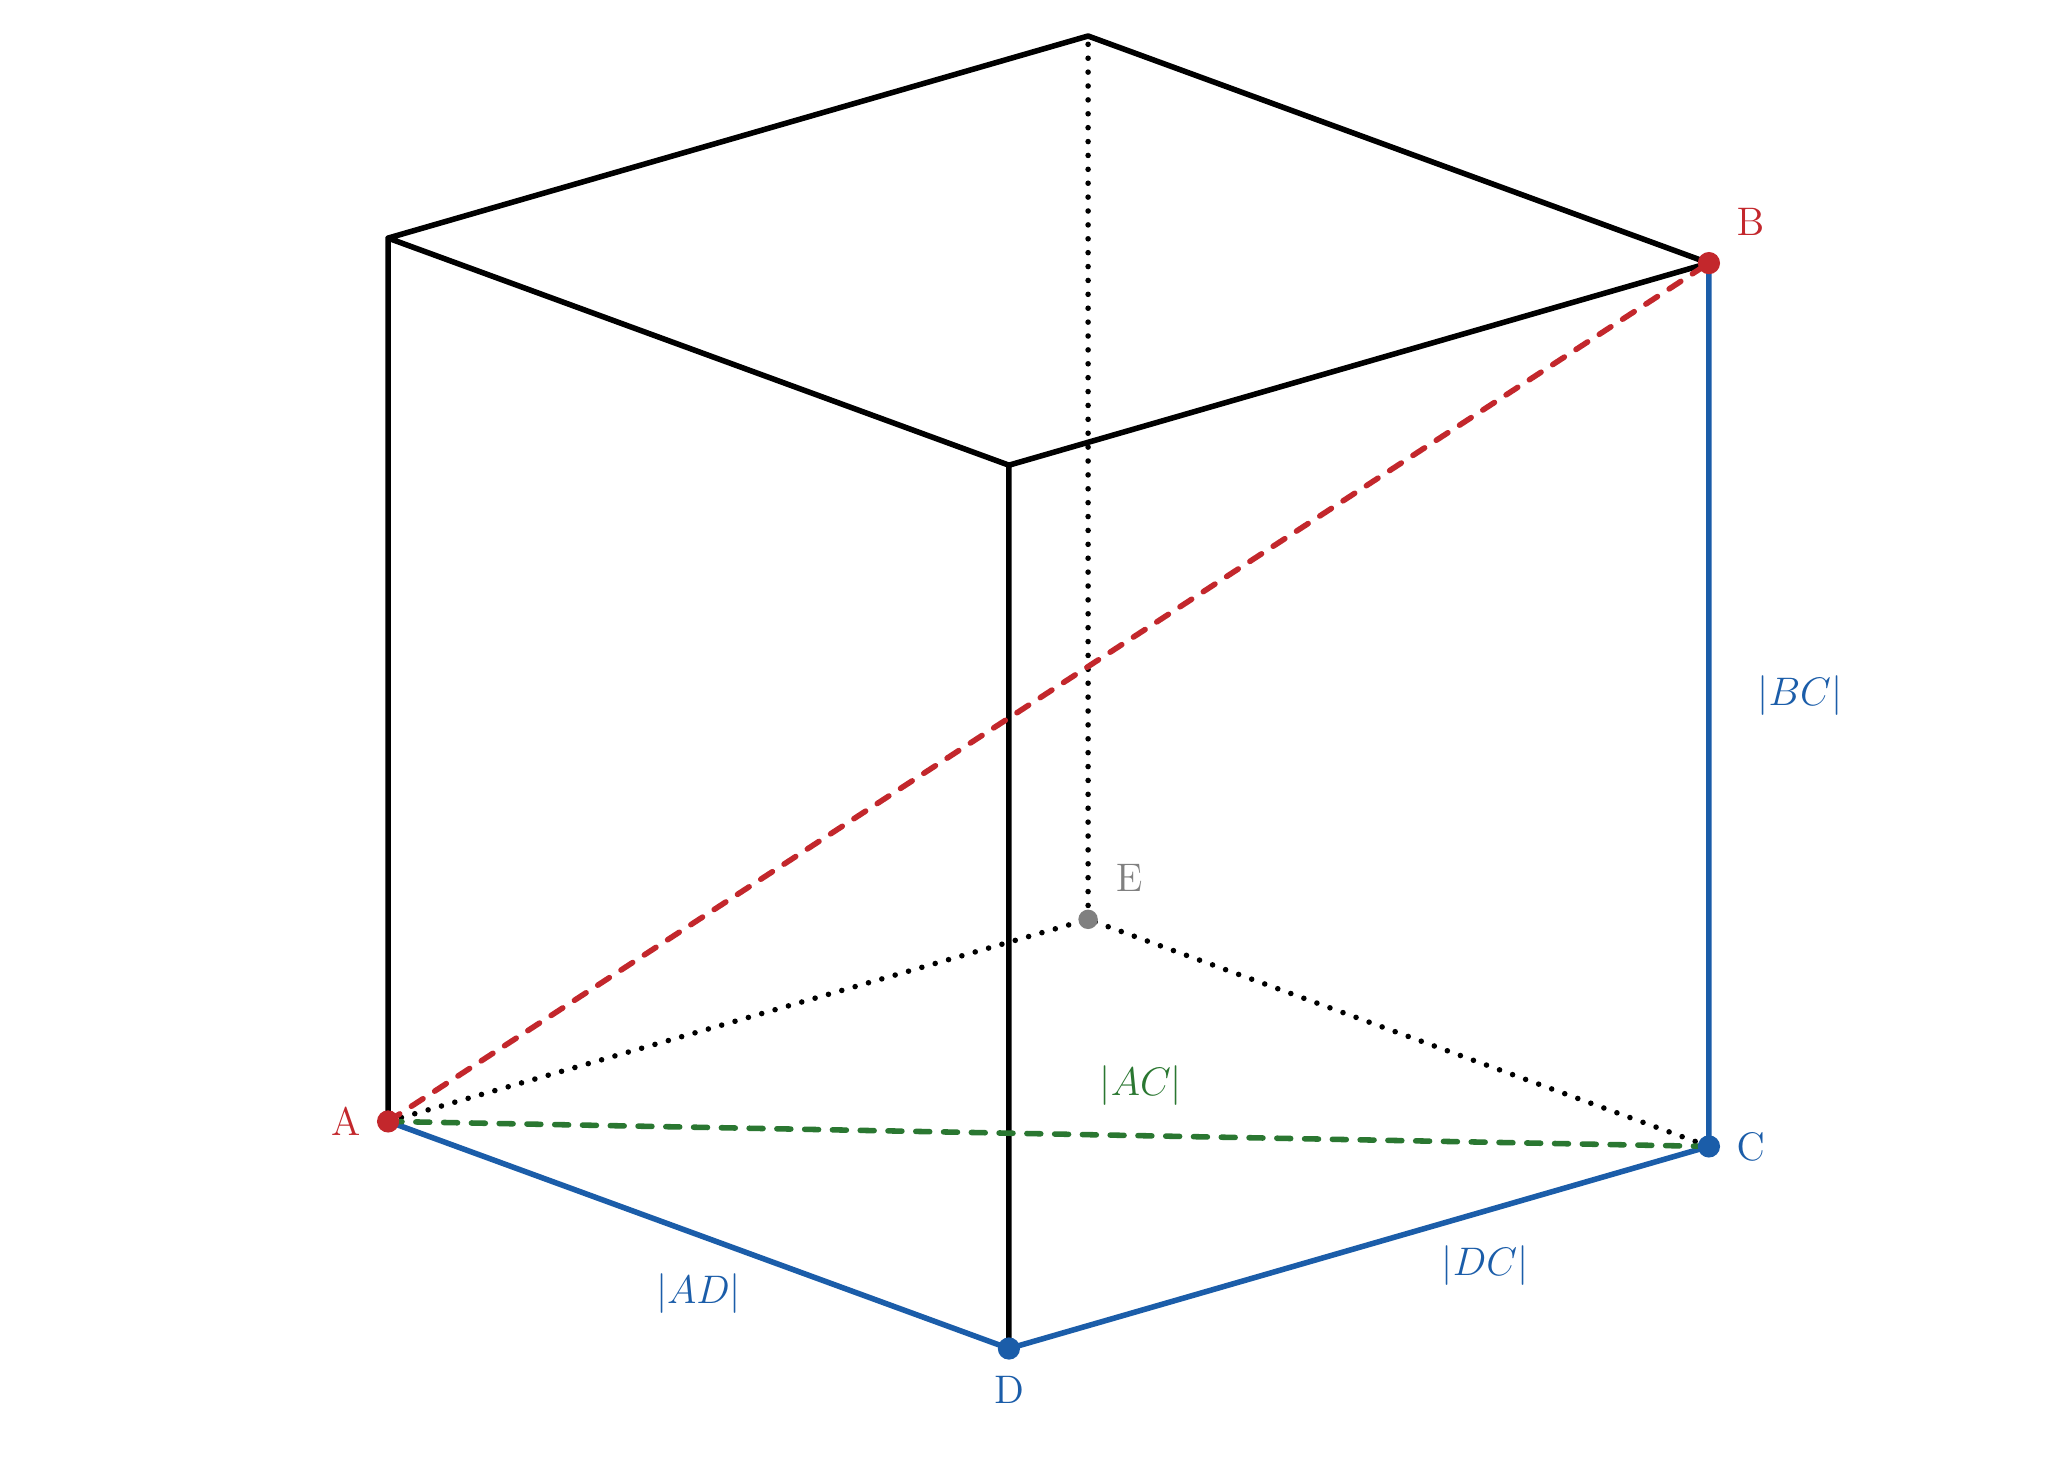
\begin{tikzpicture}[x=0.75bp,y=-0.75bp,
  line cap=round,line join=round,line width=2bp,
  every node/.style={fill=white,inner sep=3bp,font=\fontsize{14bp}{16bp}\selectfont}]
  \path[use as bounding box] (0,0) rectangle (964,680);
  \clip (0,0) rectangle (964,680);
  \fill[white] (0,0) rectangle (964,680);

  % The projected edges AD, DC and CB represent three perpendicular axes.
  % The fourth bottom vertex and the top face are derived from these edges.
  \coordinate (A) at (173,525);
  \coordinate (D) at (471,634);
  \coordinate (C) at (807,537);
  \coordinate (E) at ($(A)+(C)-(D)$);
  \coordinate (height) at (0,-424);
  \coordinate (Atop) at ($(A)+(height)$);
  \coordinate (Dtop) at ($(D)+(height)$);
  \coordinate (B) at ($(C)+(height)$);
  \coordinate (Etop) at ($(E)+(height)$);

  \draw[dash pattern=on 0bp off 5bp] (A) -- (E) -- (C) (E) -- (Etop);
  \draw (A) -- (Atop) -- (Etop) -- (B) -- (Dtop) -- (Atop)
    (D) -- (Dtop);
  \draw[edgeblue] (A) -- (D) -- (C) -- (B);
  \draw[diagonalgreen,dash pattern=on 5bp off 5bp] (A) -- (C);
  \draw[diagonalred,dash pattern=on 5bp off 5bp] (A) -- (B);

  \foreach \point in {A,B} {
    \fill[diagonalred] (\point) circle[radius=4bp];
  }
  \foreach \point in {C,D} {
    \fill[edgeblue] (\point) circle[radius=4bp];
  }
  \fill[gray] (E) circle[radius=3.5bp];

  % Draw labels last, with white backing and clearance from every edge.
  \node[text=diagonalred,left=6bp] at (A) {$\mathrm{A}$};
  \node[text=diagonalred,above right=6bp] at (B) {$\mathrm{B}$};
  \node[text=edgeblue,right=6bp] at (C) {$\mathrm{C}$};
  \node[text=edgeblue,below=6bp] at (D) {$\mathrm{D}$};
  \node[text=gray,above right=6bp] at (E) {$\mathrm{E}$};
  \node[text=edgeblue] at ($(A)!0.5!(D)+(0,28)$) {$|AD|$};
  \node[text=edgeblue] at ($(D)!0.68!(C)+(0,26)$) {$|DC|$};
  \node[text=edgeblue,anchor=west] at ($(B)!0.49!(C)+(18,0)$) {$|BC|$};
  \node[text=diagonalgreen] at ($(A)!0.57!(C)+(0,-24)$) {$|AC|$};
\end{tikzpicture}
\end{document}
